\chapter{Methodology}
\label{cha:methodology}

\section{SHMAC Setup}
\label{sec:SHMAC_setup}
In order to test the new hashing tile, and how well it scales with the system, the following setup has been set up:
\begin{itemize}
    \item Dimensions are 5x4, giving a total of 20 tiles
    \item 16 hashing tiles
    \item 2 scratchpad tiles
    \item Main memory tile and APB Interface
\end{itemize}

The setup can be seen in figure \ref{fig:5x4}.

Vexpress1 has a clock speed of 50 MHz. 

\todo{Should change away from T}
\begin{figure}[htb]
    \centering
    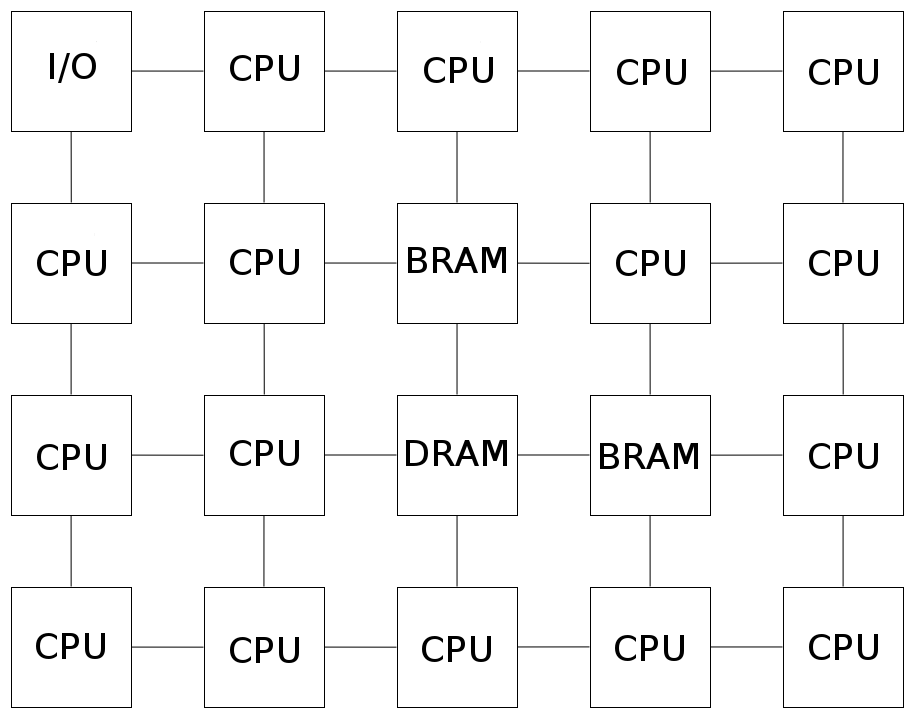
\includegraphics[width=0.5\textwidth]{Figures/Measurements/5x4}
    \caption{The SHMAC Setup. T for the CPU tiles with hashing modules, R for Scrathpad, D for Main Memory tile and V for APB interface.}
    \label{fig:5x4}
\end{figure}

\section{Measuring performance and energy efficienty}
For evaluation, the performance and energy efficiency will both be measured.
\todo{Question for Kristian: Are the counters SW-only, or on the SHA256-module?}Hashes per second are counted for each tile, and are summed together. 

Gauges for measuring is not implemented on SHMAC at this point, therefore the only way to measure the use of energy is to use a power meter plugged into the wall, that measures the power usage of the entire \todo{Not mentioned earlier}Vexpress1 computer that SHMAC runs on.

Power usage for the application running on SHMAC should be:
\newline
\newline$P_{Application} = P_{Running} - P_{Idle}$
\newline
\newline where $P_{Running}$ is the total system power consumption of Vexpress1 when running the software on SHMAC, and $P_{Idle}$ is the total system power consumption when SHMAC is idle.
The difference should indicate the power used by the application running on SHMAC.

With both performance and power measurements, energy efficiency should be calculated by\todo{Uhh.... Kristian?!!} hashes / Hz / W \textbf{(I just wrote something here, I don't remember)}

When the clock speed is taken into account, the efficiency results can be compared with other systems running at different clock speeds.

\section{Test benchmark}
Using the SHMAC setup described in \ref{sec:SHMAC_setup}, tests where run using following methods:
\begin{itemize}
    \item Hashing by software only, not using the SHA256 hashing module or DMA module.
    All operation is done on the tile processor.
    \item Hashing by using the SHA256 hashing module, but not using DMA module.
    Tile processor coordinates the hashing module, and transfers data manually.
    \item Hashing by using the SHA256 hashing module, and using DMA module for data transfer.
    Tile processor coordinates both the hashing module and the DMA module.
    \item For each setup, the measuring began with one tile, and increased, one by one, until all tiles were in use.
    \item All tiles in use are cordinated from processor tile with ID number 0, which is the first processor tile from left in the top row, seen in figure \ref{fig:5x4}.
\end{itemize}

Caches were turned on for each testing, but a bug in the caches can cause several processors to halt over time, making measurements more difficult.
Increased number of tiles in used increases the chance for a cache bug to happen.
Additionally, no cache coherency protocol is implemented, and all shared data are therefore mapped to uncachable memory.
Data hazard may be present when DMA and processor "shares" data, by loading or storing to the same address space in use.
DMA may copy outdated data from memory that the cache has not yet written back, or overwrite data that the cache is not aware of.
An operating system may handle data coherency where DMA involved, but since this project is done by running the software on bare metal, this security is absent.
The Turbo Amber processor uses \todo{Must get it confirmed, and then source linked}write-through policy, so every data update is always written back to memory, \todo{Want to mention "reduced, but not removed", due to how our tests may go} reducing the possibility of data hazard, but not removing it.

Interrupt handling for the hashing module is always in use, when the accelerator is used.

The DMA Module is made only for transfering 32-bit words individually at a time.
When transferring data internal on the tile (regular tile registers, hashing registers and DMA registers), this is all the local system requires, as the tile modules does not provide full blocks of \todo{Use of wishbone, with size 128, is not yet provided}4 words.
\todo{Merely an assumption. We haven't tested this.}But when running the hashing in software only, the system is likely to achieve better data transfer rate using regular processor data transfer of 4 words, through the caches, since the current DMA would require 4 individual transfer, compared to the processor.

The use of the included sub-module in the DMA that moves the bytes from high endian to little endian should further improve the performance and energy efficiency, by relieving the software for this task.
The byte flip is done through combinatorical circuits, and should not add any extra execution time.
Wihtout it, the software would require several independent operations, for loading in and shifting every single byte to the correct position of the word.

Additionally, polling is used to control when a DMA is finished.
Ideally, interrupt handling is preferable, but the interrupt handler for the DMA would not \todo{yet}work. 